\subsection{Számlálók}

%_
\begin{frame}
  Számlálók: mint egy program változói, melyek értéke változik (ált. nő) a használat hatására\\
  Használható pl. fejezetek vagy felsorolások számozására
  \vfill
  \texttt{counter-reset}: számláló létrehozása, újraindítása vagy kezdőértékkel ellátása.
  \begin{description}[m]
    \item[\texttt{none}] \hfill \\ Számlálók nem lesznek inicializálva, alapértelmezés.
    \item[\texttt{id number}] \hfill \\ Az \emph{id} azonosítójú számláló felveszi a \emph{number} értéket. Utóbbi elhagyható, alapértelmezetten 0.
  \end{description}
\end{frame}

%_
\begin{frame}
  \texttt{counter-increment}: számláló értékének léptetése
  \begin{description}[m]
    \item[\texttt{none}] \hfill \\ Nem változtat a számlálók értékén, alapértelmezés.
    \item[\texttt{id number}] \hfill \\ Hozzáad \emph{number}-t (alapértelmezetten 1, de lehet akár negatív érték is) az \emph{id} számláló értékéhez. 
  \end{description}
  \vfill
  A \texttt{content} tulajdonságot használják a számlálók értékének kijelzésére, jellemzően a \texttt{::before} látszóleges elemben (\hiv{\href{https://developer.mozilla.org/en-US/docs/Web/CSS/::marker}{\texttt{::marker}}} gyengén támogatott). Ugyanitt ált. számláló növelésre is sor kerül.
\end{frame}

%_
\begin{frame}
  \texttt{counter(id)} vagy \texttt{counter(id, style)}: számláló értékének lekérdezése
  \begin{description}[m]
    \item[\texttt{id}] \hfill \\ A \texttt{counter-reset}-tel létrehozott és \texttt{counter-increment}-tel léptetett változó azonosítója.
    \item[\texttt{style}] \hfill \\ A számláló megjelenítési módja, pl. \texttt{lower-alpha}, \texttt{upper-roman}, \texttt{decimal-leading-zero}, stb., vagy a \hiv{\href{https://developer.mozilla.org/en-US/docs/Web/CSS/symbols}{\texttt{symbols()}}} függvénnyel adott szimbólumok.
  \end{description}
\end{frame}

%_
\begin{frame}
  \begin{columns}[c]
    \column{0.5\textwidth}
      \begin{exampleblock}{\textattachfile{szamozottFejezet.html}{szamozottFejezet.html}}
        \scriptsize
        \lstinputlisting[style=HTML,linerange={7-16},numbers=left,firstnumber=7]{szamozottFejezet.html}
      \end{exampleblock}
    \column{0.5\textwidth}
      \begin{exampleblock}{}
        \scriptsize
        \lstinputlisting[style=HTML,linerange={19-28},numbers=right,firstnumber=19]{szamozottFejezet.html}
      \end{exampleblock}
  \end{columns}
\end{frame}

%_
\begin{frame}
  \begin{center}
    
\includegraphics[width=.5\textwidth]{szamozottFejezet.png}\\
    \textattachfile{szamozottFejezet.html}{szamozottFejezet.html}
  \end{center}
\end{frame}

%_
\begin{frame}
  Egymásba ágyazott azonos típusú elemeknél (pl. \texttt{<ol>}, \texttt{<ul>}) rekurzívan mindig új számláló keletkezik. Megjelenítésük: \texttt{counters(id, string)} vagy \texttt{counters(id, string, style)} függvénnyel.
  \begin{description}[m]
    \item[\texttt{id}] \hfill \\ A számláló neve.
    \item[\texttt{string}] \hfill \\ A számlálók értékeit elválasztó karakterlánc.
    \item[\texttt{style}] \hfill \\ A számlálók stílusa.
  \end{description}
\end{frame}

%_
\begin{frame}
  \begin{columns}[c]
    \column{0.54\textwidth}
      \begin{exampleblock}{\textattachfile{szamozottLista.html}{szamozottLista.html}}
        \scriptsize
        \lstinputlisting[style=HTML,linerange={7-16},numbers=left,firstnumber=7]{szamozottLista.html}
      \end{exampleblock}
    \column{0.43\textwidth}
      \begin{exampleblock}{}
        \scriptsize
        \lstinputlisting[style=HTML,linerange={21-31},numbers=right,firstnumber=21]{szamozottLista.html}
      \end{exampleblock}
  \end{columns}
\end{frame}

%_
\begin{frame}
  \begin{center}
    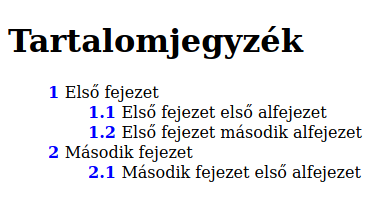
\includegraphics[width=.5\textwidth]{szamozottLista.png}\\
    \textattachfile{szamozottLista.html}{szamozottLista.html}
  \end{center}
\end{frame}

%_
\begin{frame}
  \begin{columns}[c]
    \column{0.8\textwidth}
      Készítse el a mellékelt \textattachfile{teendok.html}{teendok.html} oldalt!
      \begin{itemize}
        \item A kétszintű felsorolás külső szintjén alkalmazzon nagybetűs római számokat, a belsőn arab számokat!
        \item Utóbbiak számozása az egész oldalon legyen folytonos (1-6)!
        \item A számokat helyezze sárga hátterű ellipszisek közepébe, kék színnel és félkövér betűkkel megjelenítve!
      \end{itemize}
    \column{0.15\textwidth}
      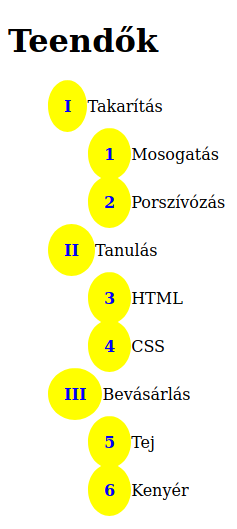
\includegraphics[width=\textwidth]{teendok.png}
  \end{columns}
\end{frame}
